\section{Cas d'Utilisation}
Pour schématiser les besoins fonctionnels, nous avons recours au diagramme de cas d'utilisation d'UML (Unified Modeling Language), qui décrit les interactions entre les acteurs et le système.

\subsection{Identification des Acteurs}
Un acteur représente l'entité qui interagit avec le système. Dans notre projet, nous avons identifié deux acteurs principaux et un acteur système :
\begin{itemize}
    \item \textbf{L'athlète (Sportif)} : Utilisateur principal de l'application mobile.
    \item \textbf{Le coach (Professionnel)} : Utilisateur gérant ses clients via l'espace pro.
    \item \textbf{Le système (IA Backend/Mobile)} : Déclenche les analyses vidéo et l'adaptation des programmes en tâche de fond.
\end{itemize}

\subsection{Modélisation par Domaine}
Pour une meilleure lisibilité et une compréhension fine du système, nous avons structuré nos diagrammes de cas d'utilisation autour de trois domaines fondamentaux de l'application, subdivisés en pôles métiers.

\subsubsection{1. Domaine Sportif : L'Expérience Athlète}

\paragraph{Pôle Entraînement et Exécution}
Ce sous-système représente le cœur de l'action pour le sportif au sein de la plateforme SmartFit. Il illustre le processus de déclenchement d'une séance d'entraînement et l'enregistrement continu de l'historique d'activité. Afin d'offrir une expérience d'entraînement enrichie et sécurisée, ce module s'appuie sur des extensions technologiques majeures : le suivi GPS pour cartographier les activités en extérieur, et l'intégration de modèles d'Intelligence Artificielle dédiés à la détection de posture en temps réel pour optimiser l'exécution des mouvements.
\begin{figure}[H]
    \centering
    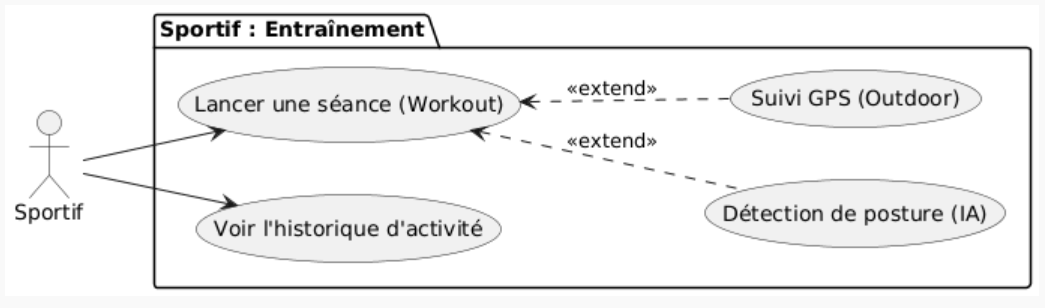
\includegraphics[width=0.8\textwidth]{img/use-case/1-a.png}
    \caption{Diagramme de Cas d'Utilisation : Pôle Entraînement et Exécution}
\end{figure}

\paragraph{Pôle Suivi, Nutrition et Coaching}
Ce module se concentre sur l'accompagnement continu de l'athlète en dehors de ses sessions actives. Il détaille l'accès au tableau de bord (dashboard) centralisant les métriques de performance, le suivi quotidien de la nutrition, ainsi que les interfaces de recherche et de communication. Ce pôle garantit que l'utilisateur dispose de tous les outils nécessaires, de la diététique à la discussion directe avec un coach, pour atteindre ses objectifs au sein d'un environnement unifié.
\begin{figure}[H]
    \centering
    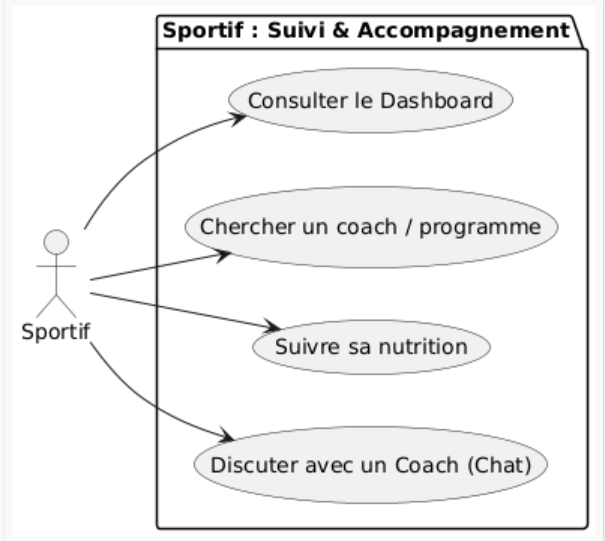
\includegraphics[width=0.8\textwidth]{img/use-case/1-b.png}
    \caption{Diagramme de Cas d'Utilisation : Pôle Suivi, Nutrition et Coaching}
\end{figure}

\subsubsection{2. Domaine Coach : L'Espace Professionnel}

\paragraph{Pôle Création de Contenu}
Réservé aux professionnels du sport, ce sous-système modélise le travail de conception pédagogique. Il permet aux coachs de constituer leur propre base de données métier en créant des exercices isolés détaillés, puis en les assemblant de manière logique pour concevoir des programmes d'entraînement complets et personnalisables, prêts à être déployés auprès de leurs athlètes.
\begin{figure}[H]
    \centering
    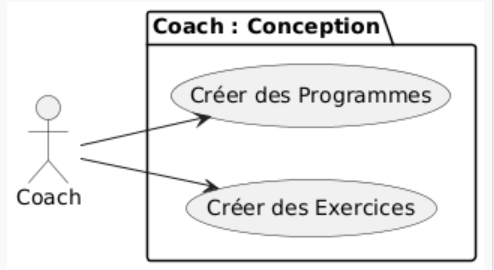
\includegraphics[width=0.8\textwidth]{img/use-case/2-a.png}
    \caption{Diagramme de Cas d'Utilisation : Pôle Création de Contenu}
\end{figure}

\paragraph{Pôle Gestion de la Clientèle et Pilotage}
Ce pôle regroupe les fonctionnalités de gestion de la relation client (CRM) et de pilotage analytique. Il illustre la manière dont le coach supervise sa base d'utilisateurs, gère son emploi du temps via un agenda intégré, et communique avec ses clients. La consultation des Analytics et le suivi régulier des progrès sont au centre de ce module, permettant au professionnel d'adopter une approche d'accompagnement basée sur la donnée (data-driven).
\begin{figure}[H]
    \centering
    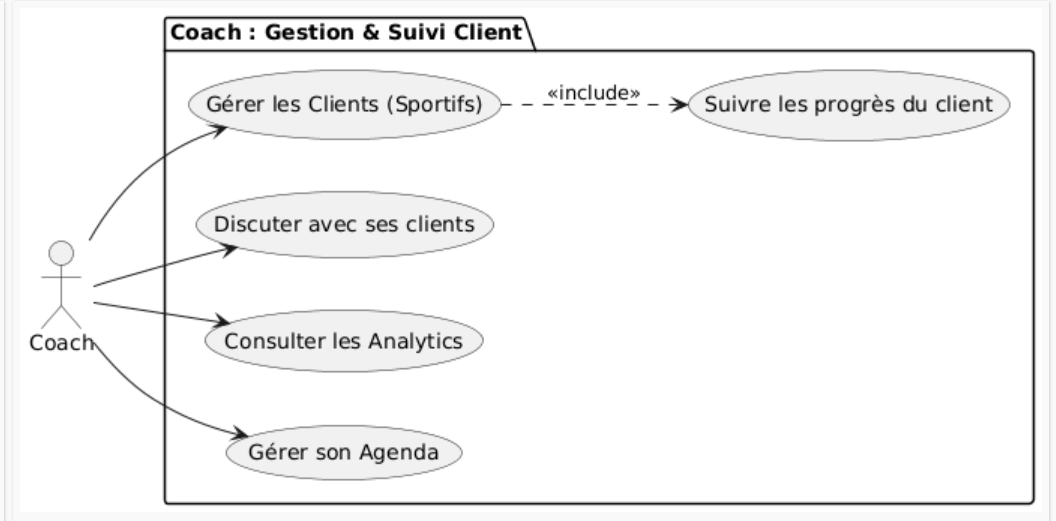
\includegraphics[width=0.8\textwidth]{img/use-case/2-b.png}
    \caption{Diagramme de Cas d'Utilisation : Pôle Gestion de la Clientèle et Pilotage}
\end{figure}

\subsubsection{3. Domaine Sécurité \& Onboarding}

\paragraph{Pôle Accès et Sécurité}
Ce module standardise le point d'entrée du système pour tout visiteur. Il couvre les cas d'utilisation fondamentaux liés à la gestion des accès et à la sécurité : la création d'un compte (inscription), l'authentification sécurisée (connexion), ainsi que les procédures de récupération en cas de perte de mot de passe, assurant ainsi la protection stricte des données personnelles des utilisateurs. L'utilisateur doit d'abord passer par le cas d'utilisation \textit{S'authentifier} (relation \texttt{<<include>>}) pour accéder aux autres fonctionnalités sécurisées.
\begin{figure}[H]
    \centering
    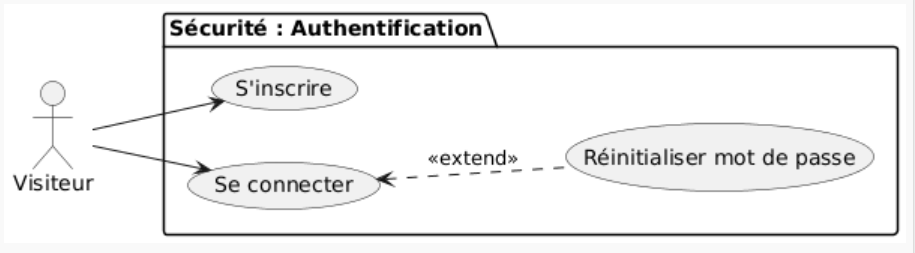
\includegraphics[width=0.8\textwidth]{img/use-case/3-a.png}
    \caption{Diagramme de Cas d'Utilisation : Pôle Accès et Sécurité}
\end{figure}

\paragraph{Pôle Profil \& Onboarding}
Étape cruciale suivant la création du compte, ce sous-système modélise la phase d'intégration (onboarding) et le paramétrage initial. La configuration du profil inclut obligatoirement la saisie des mensurations initiales et des objectifs physiques de l'utilisateur. Cette étape est indispensable pour amorcer l'algorithme de la plateforme et permettre aux coachs de proposer un suivi sur-mesure dès les premiers jours d'utilisation.
\begin{figure}[H]
    \centering
    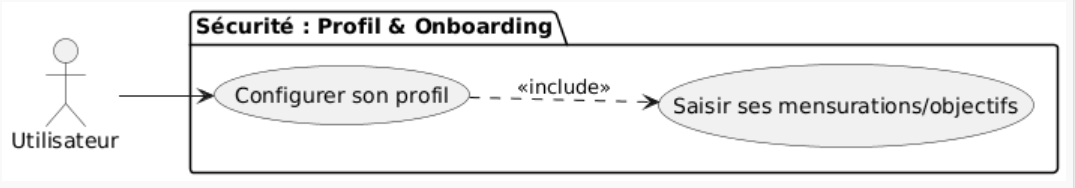
\includegraphics[width=0.8\textwidth]{img/use-case/3-b.png}
    \caption{Diagramme de Cas d'Utilisation : Pôle Profil \& Onboarding}
\end{figure}
